\begin{frame}{Why develop BCDI at SixS}
    \begin{columns}
        \column[T]{0.65\textwidth}
            \begin{itemize}
                \item Complementary with Surface X-Ray Diffraction \pause
                \item Same reactor cell allowing \textit{in-situ} and \textit{operando} experiments at ambient pressure followed with a mass spectrometer
            \end{itemize}
            \pause 
            
            \begin{figure}
                \centering
                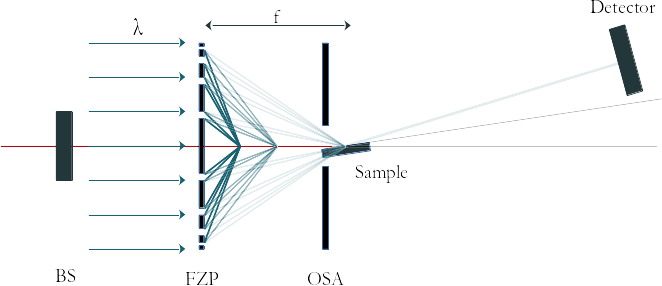
\includegraphics[width=\textwidth]{Figures/sixs/optical_setup.png}
                \caption{Optical elements improve the coherent flux on the sample.}
                \label{fig:optical_setup}
            \end{figure}
            \pause

            \begin{tabular}{l|l|l|l|l}
                 & Beam stop & FZP & OSA & Beam\\ \hfill
                Diameter $\Omega$ & $80 \, \mu m$ & $300 \, \mu m$ & $70 \, \mu m$ & $\approx 1 \, \mu m$\\
            \end{tabular}
            \pause

        \column{0.3\textwidth}
            \begin{figure}
                \centering
                \includegraphics[width=\textwidth]{Figures/sixs/CELL.jpg}
                \caption{Reactor cell and dome}
                \label{fig:CELLDome}
                \bigskip
                \pause
                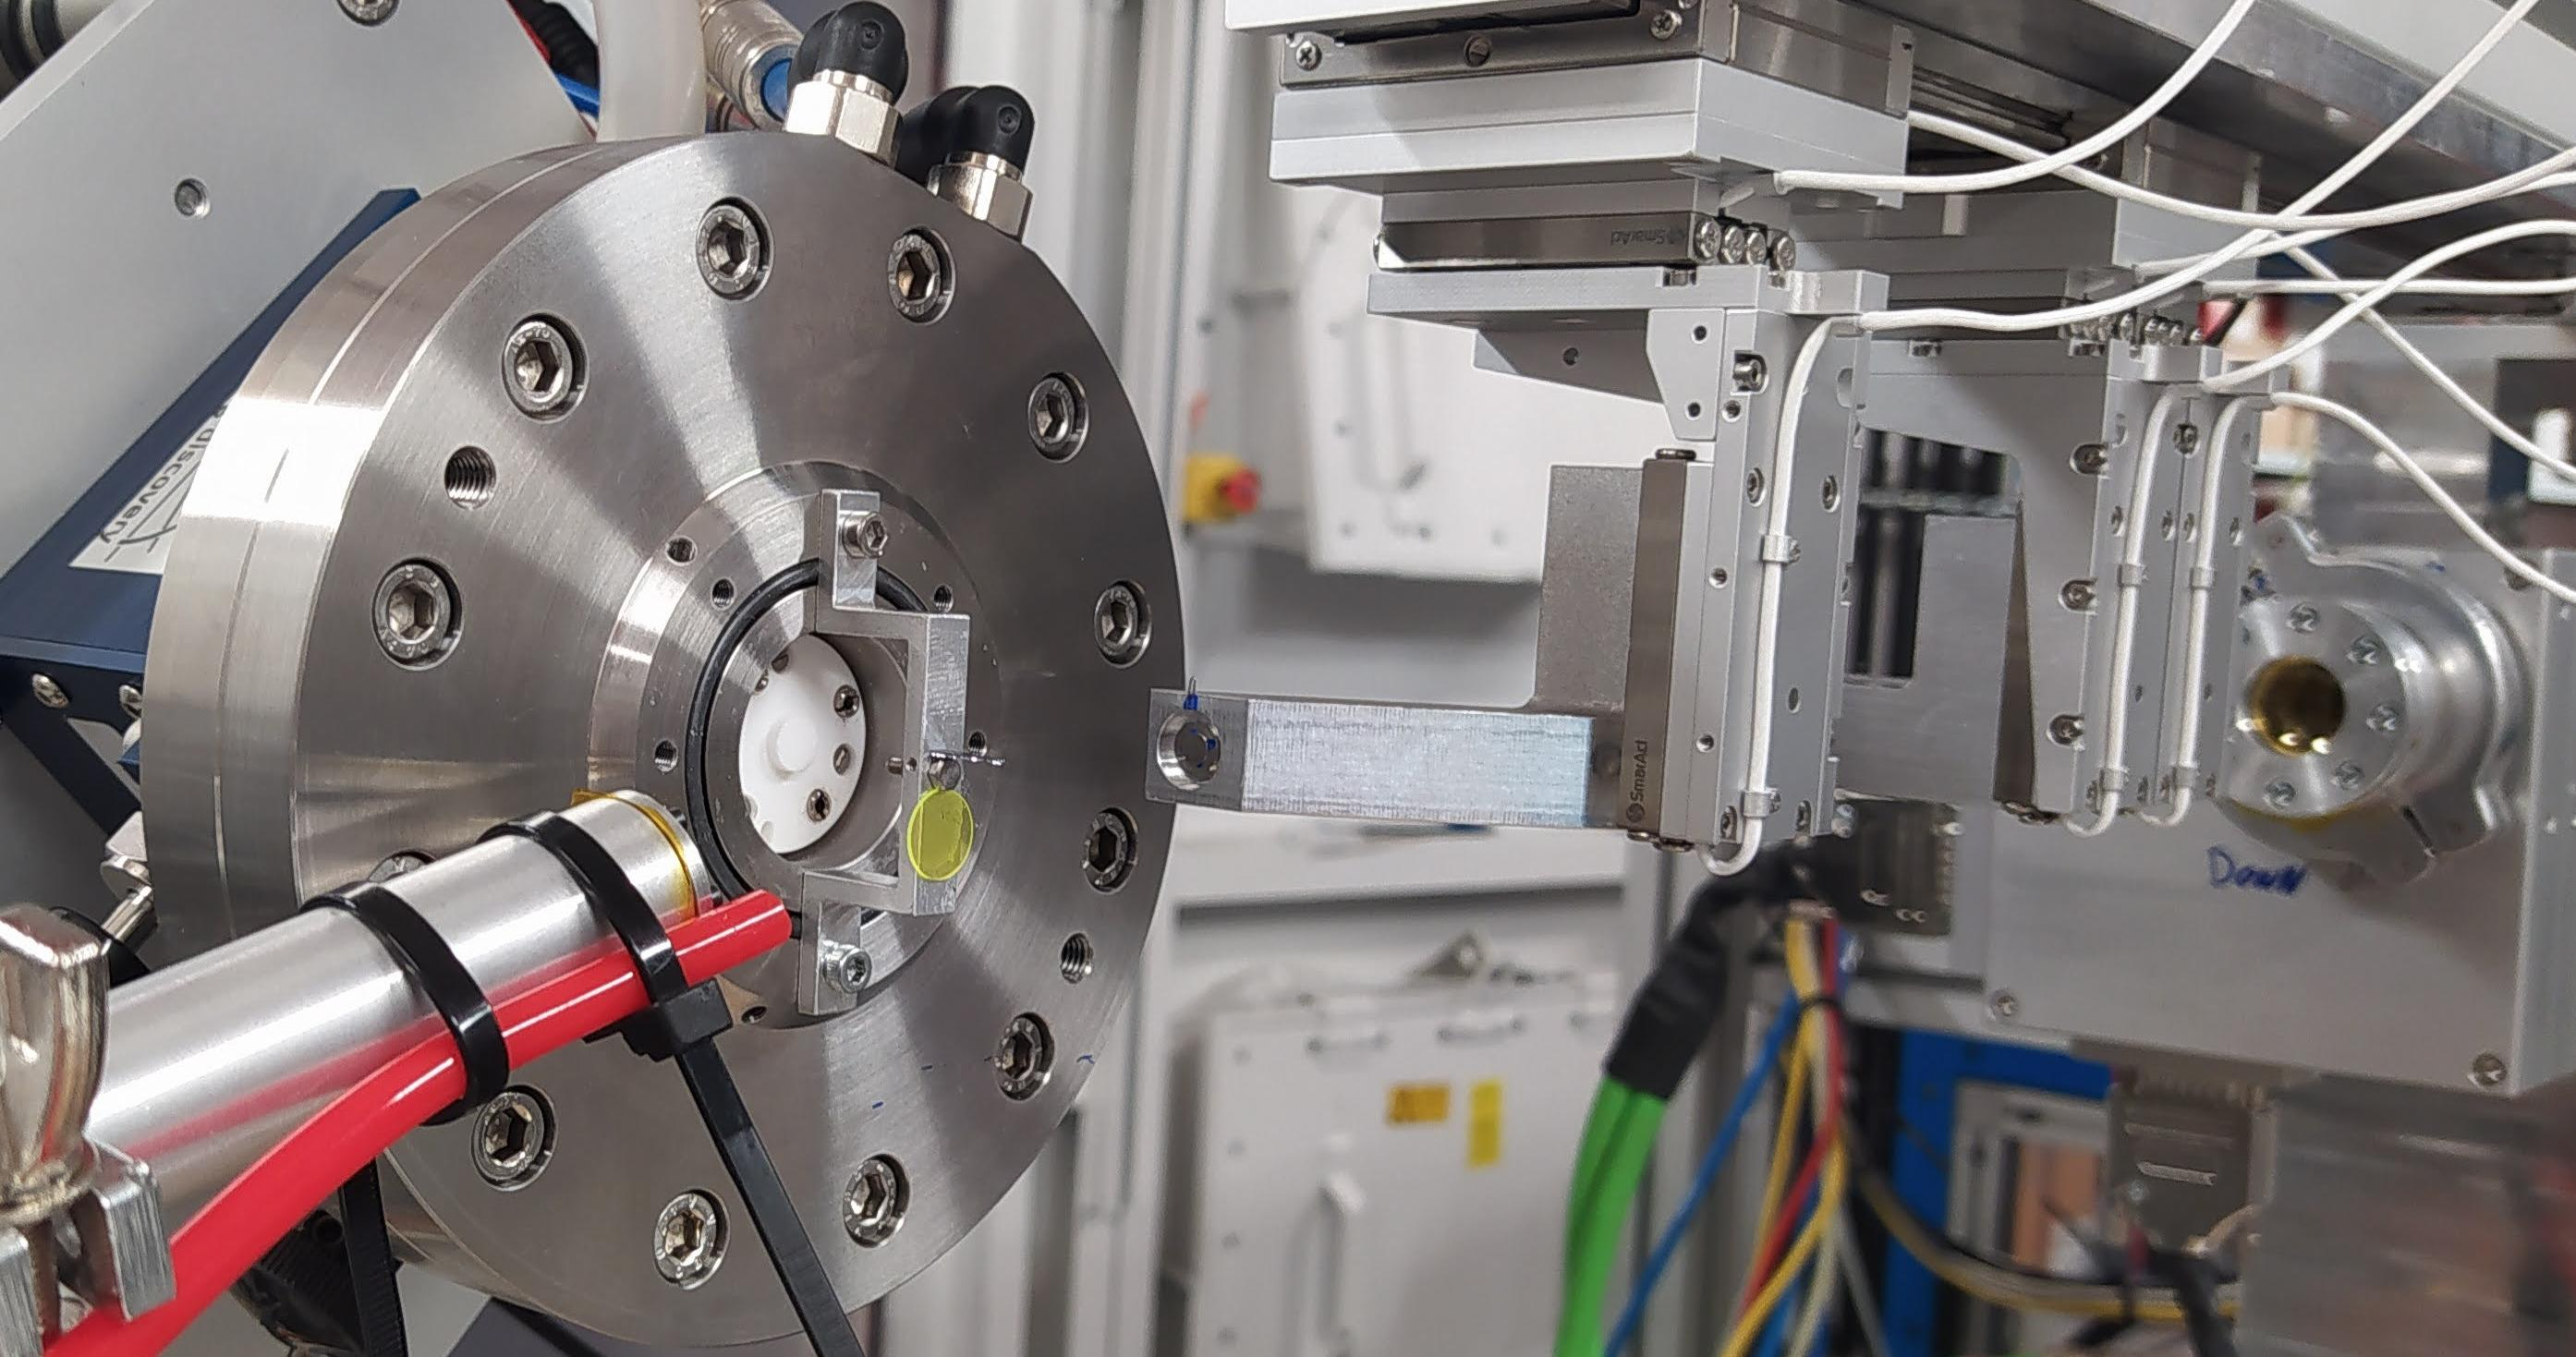
\includegraphics[width=\textwidth]{Figures/sixs/opt_elements_photo.jpg}
                \caption{Coherence slits → beam stop (BS) → Fresnel zone plates (FZP) → order selecting aperture (OSA) → XCAT reactor}
                \label{fig:3Doptics}
            \end{figure}

    \end{columns}
\end{frame}